% hablamos de la aplicación

\begin{frame}
	\frametitle{La aplicación \ULLAR{}}
	\block{Requisitos de \ULLAR{}}
	\begin{itemize}
		\item La aplicación se desarrollará para dispositivos con Android. 
		\item Se implementarán técnicas de realidad aumentada basadas en la geolocalización.
		\item El servidor y base de datos de la aplicación estarán alojados en la nube.
	\end{itemize}
	\endblock{}
\end{frame}


\begin{frame}
	\centering{Vídeo demostrativo de la aplicación \ULLAR{}} 
\end{frame}

%--------------------------------------------------------------------

% \begin{frame}
% 	\frametitle{Asociación de MAC a identificador de }
% 	\lstinputlisting{Code/BeaconBusStop.java}
% \end{frame}

%--------------------------------------------------------------------
% Explicación activity y layout
%--------------------------------------------------------------------

\begin{frame}
	\frametitle{Inicio de la aplicación}
	\begin{columns}
		\begin{column}{0.6\textwidth}
			\block{Splash Screen}
			\begin{itemize}
				\item Logo de \ULLAR{}.
				\item Mejor apariencia.
				\item Pantalla de carga de la aplicación.
			\end{itemize}
			\endblock{}
		\end{column}
		\begin{column}{0.4\textwidth}
			\vfill 
			\begin{center}
				
\includegraphics[width=0.7\linewidth]{Images/splashApp}
			\end{center}
		\end{column}
	\end{columns}
\end{frame}

%--------------------------------------------------------------------
 

\begin{frame}
	\frametitle{Inicio de la aplicación}
	\begin{columns}
		\begin{column}{0.6\textwidth}
			\block{Ventana de  \textit{Inicio de Sesión}}
			\begin{itemize}
				\item Permitir al usuario identificarse con su cuenta de la ULL.
				\item Uso API de Google.
				\item Integrada en Firebase.
			\end{itemize}
			\endblock{}
		\end{column}
		\begin{column}{0.4\textwidth}
			\vfill 
			\begin{center}
				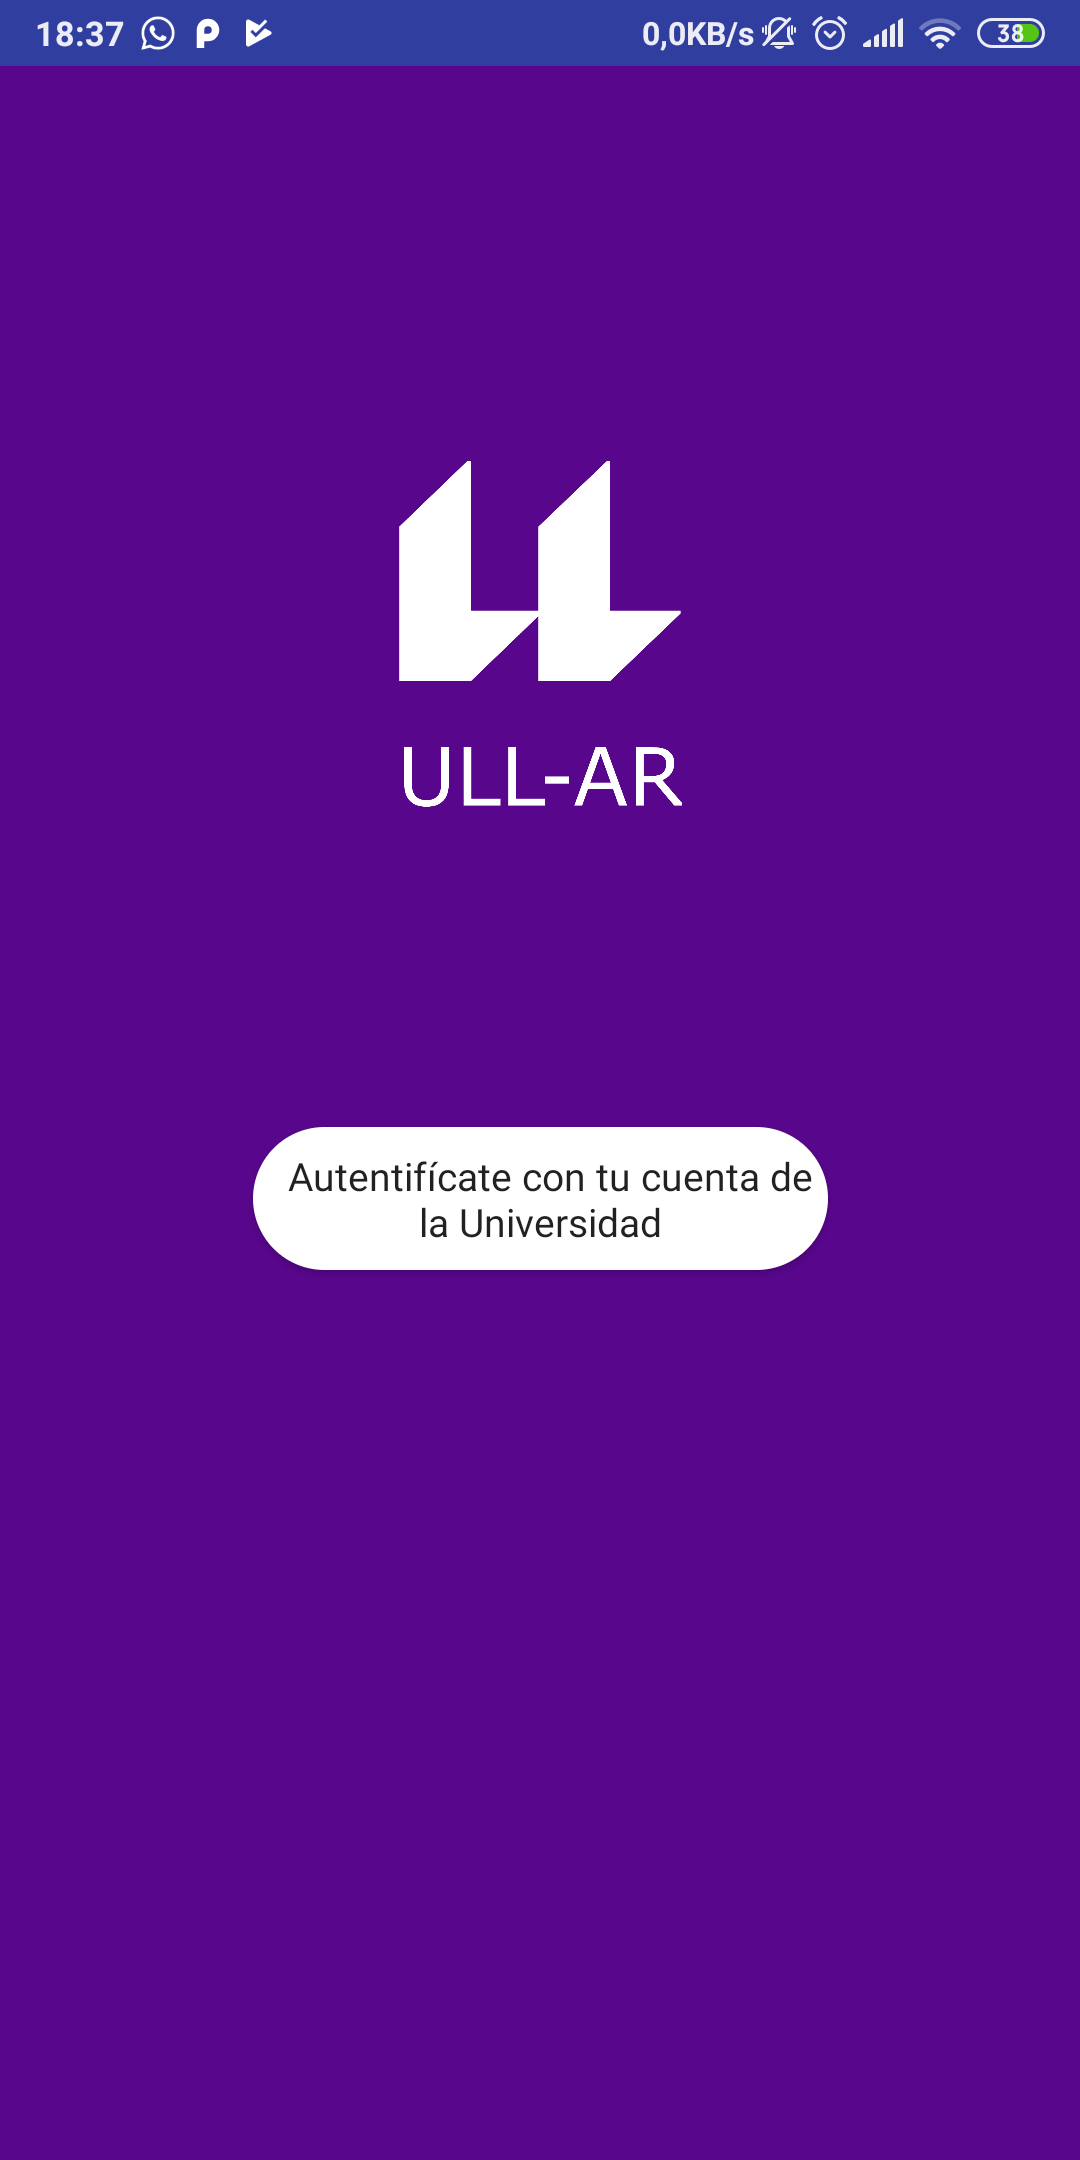
\includegraphics[width=0.7\linewidth]{Images/loginApp}
			\end{center}
		\end{column}
	\end{columns}
\end{frame}
  
 
\begin{frame}
	\frametitle{Ventana de  \textit{Inicio de Sesión}}
	\lstinputlisting{Code/login1.java}
\end{frame}


\begin{frame}
	\frametitle{Ventana de  \textit{Inicio de Sesión}}
	\lstinputlisting{Code/login2.java}
\end{frame}
%------------------------------------- -------------------------------

\begin{frame}
	\frametitle{Modo de Realidad Aumentada}
	\begin{columns}
		\begin{column}{0.6\textwidth}
			\block{Ventana de  \textit{Navegación en modo RA}}
			\begin{itemize}
				\item RA basada en geolocalización.
				\item Acceso a los sensores del dispositivo.
				\item Identificación de las instalaciones de la ULL.
				\item Obtencion de las instalaciones.
				\item La clase ARNavigation.java es el activity principal encargado.
			\end{itemize}
			\endblock{}
		\end{column}
		\begin{column}{0.4\textwidth} 
			\vfill 
			\begin{center}
				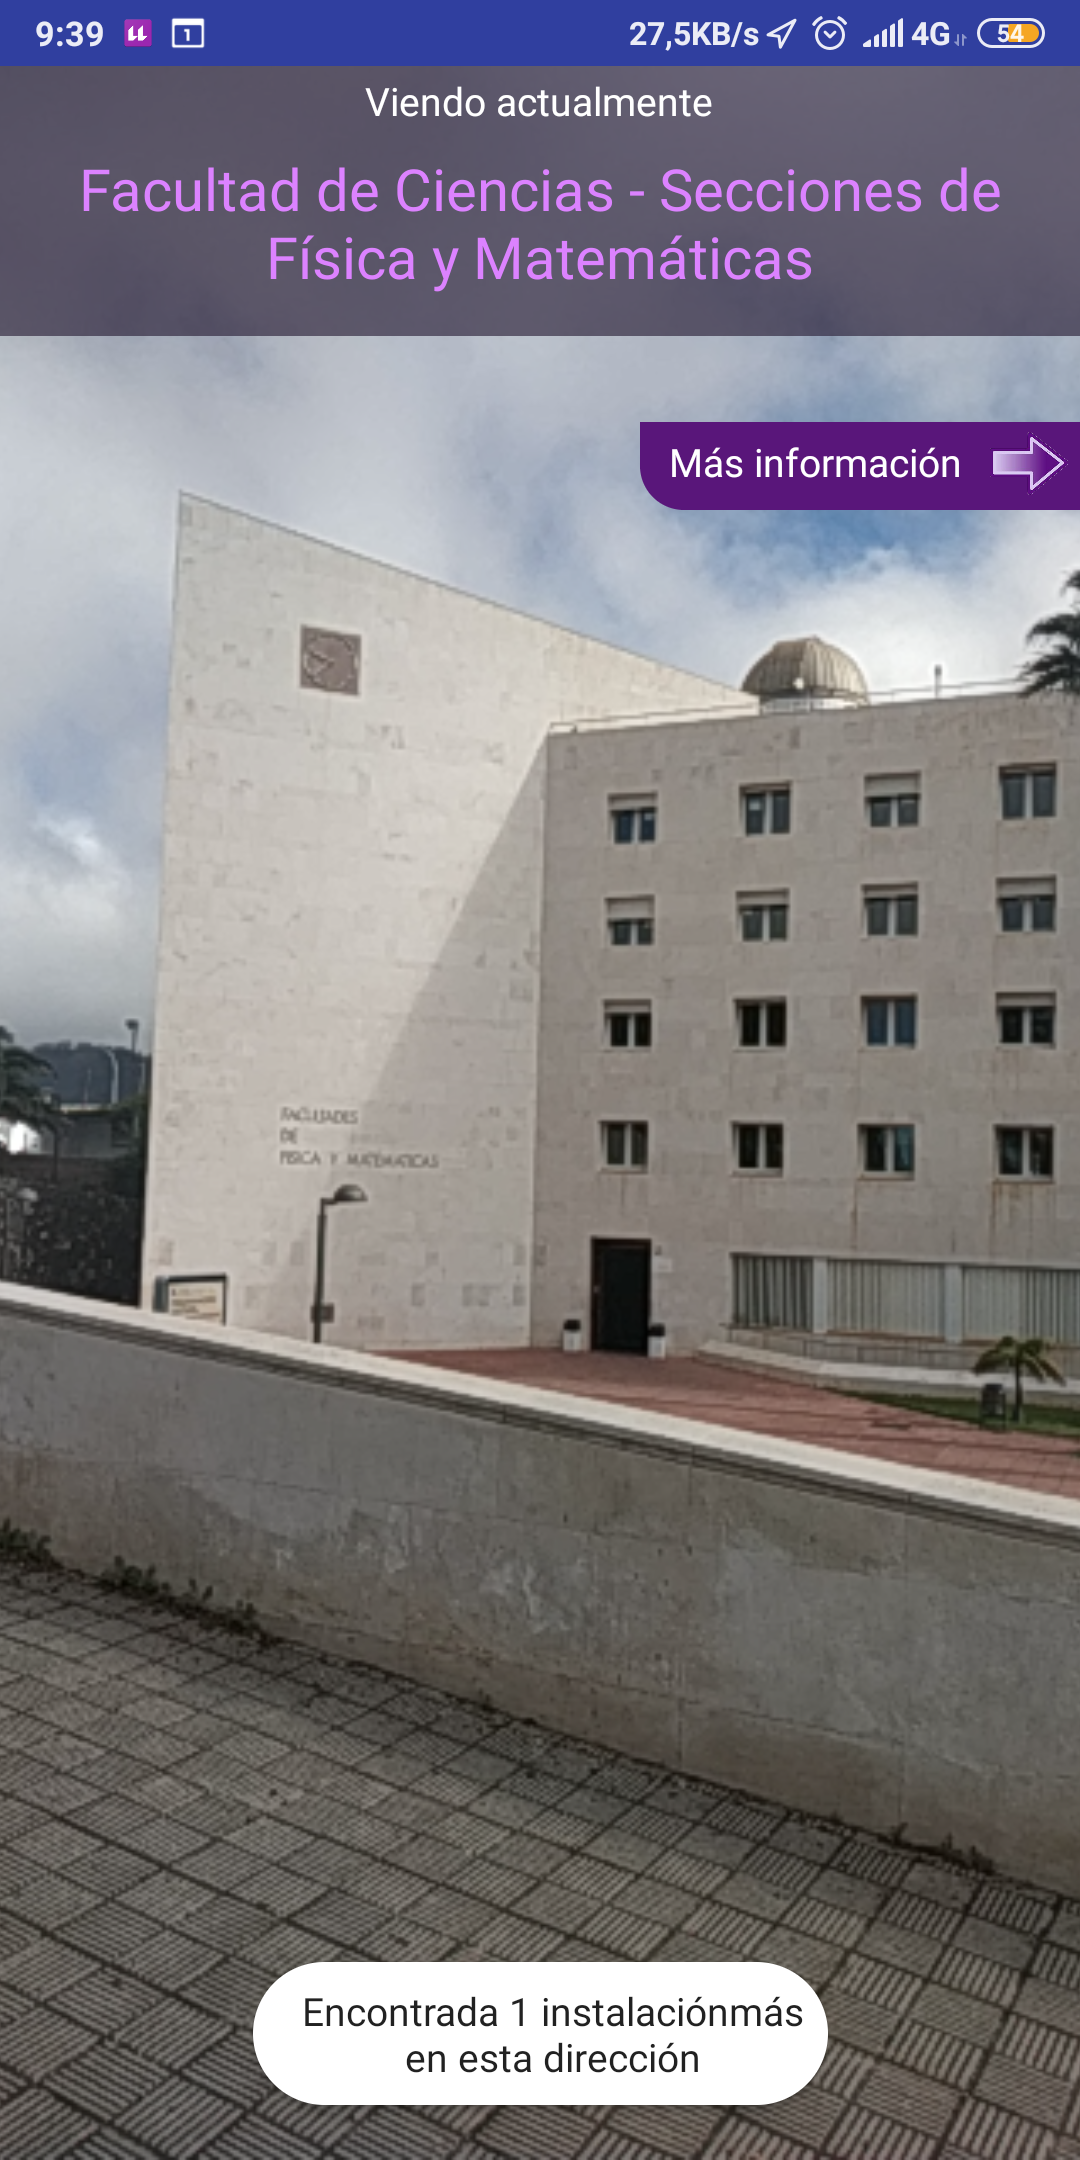
\includegraphics[width=0.7\linewidth]{Images/ar}
			\end{center}
		\end{column}
	\end{columns}
\end{frame}

 
\begin{frame}
	\frametitle{Acceso a la ubicación del dispositivo}
	\texttt{AndroidManifest.xml}
	\lstinputlisting{Code/permisosgps.xml}

	\texttt{ARNavigation.java}
	\lstinputlisting{Code/permisosgps2.java}
\end{frame}
%--------------------------------------------------------------------


 
\begin{frame}
	\frametitle{Acceso a la orientación del dispositivo}
	\lstinputlisting{Code/permisosgps3.java}
	\lstinputlisting{Code/permisosgps4.java}
\end{frame}



\begin{frame}
	\frametitle{Acceso a la orientación del dispositivo}
	\block{Orientación de un dispositivo Android}
	\begin{itemize}
		\item Matriz de rotación que Android calcula a partir de magnetómetro y el acelerómetro. 
		\item Se obtiene el valor de brújula magnética del dispositivo.
		\item Permite orientar al dispositivo en el espacio para poder identificar las instalaciones.
	\end{itemize}
	\endblock{}
	\lstinputlisting{Code/brujula.java}
\end{frame}


 


\begin{frame}
	\frametitle{Acceso a la orientación del dispositivo}
		\block{Orientación de un dispositivo Android}
			\begin{itemize}
				\item Android dispone de 3 ejes: x, y, z.
				\item Valor de acimut.
				\item Obtención de la orientación del dispositivo con respecto al norte magnético.
			\end{itemize}
		\endblock{}

		\begin{center} 
			\hspace*{0.5in}
			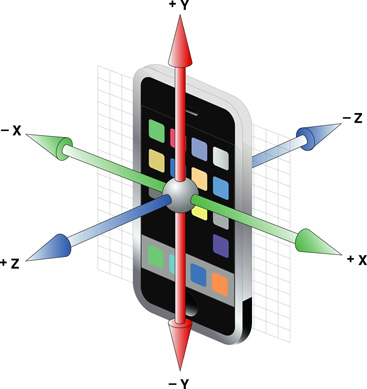
\includegraphics[width=0.3\linewidth]{Images/xyz}
			\hfill
			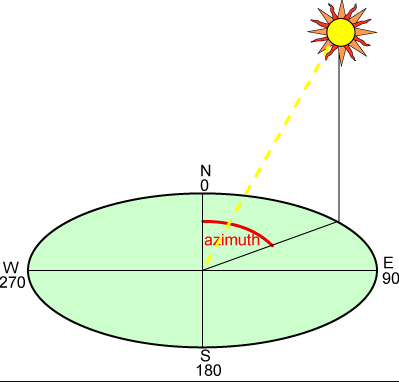
\includegraphics[width=0.3\linewidth]{Images/acimut}
			\hspace*{0.5in}
		\end{center}
\end{frame}		
		

\begin{frame}
	\frametitle{Acceso a la orientación del dispositivo}
	\lstinputlisting{Code/brujula2.java}
\end{frame}


\begin{frame}
	\frametitle{Modo de Realidad Aumentada}
			\block{Modelos encargados de la navegación}
			Clases que intervienen:
			\begin{itemize}
				\item \texttt{ULLSite.java}
				\item \texttt{Navigation.java}
				\item \texttt{Vector2D.java}
			\end{itemize}
			\endblock{}

			\block{\texttt{ULLSite.java}}
			\begin{itemize}
				\item Almacena la información referente a una instalación de la ULL.
				\item Se crea a partir del objeto JSON contenido en la base de datos.
				\item Contiene los atributos que permiten identificar una instalación.
			\end{itemize}
			\endblock{}

\end{frame}
 
\begin{frame}
	\frametitle{Objeto JSON con la información de una instalación}
	\lstinputlisting{Code/ull_site.json}
\end{frame}

\begin{frame}
	\frametitle{\texttt{ULLSite.java}}
	\lstinputlisting{Code/ULLSite.java}
\end{frame}


\begin{frame}
	\frametitle{\texttt{ULLSite.java}}
			\block{Principales atributos que intervienen en la navegación}
			\begin{itemize}
				\item  ``disToSite''
				\item ``dirToSite''
				\item ``coneValue''
			\end{itemize}
			\endblock{}
			\begin{center} 
				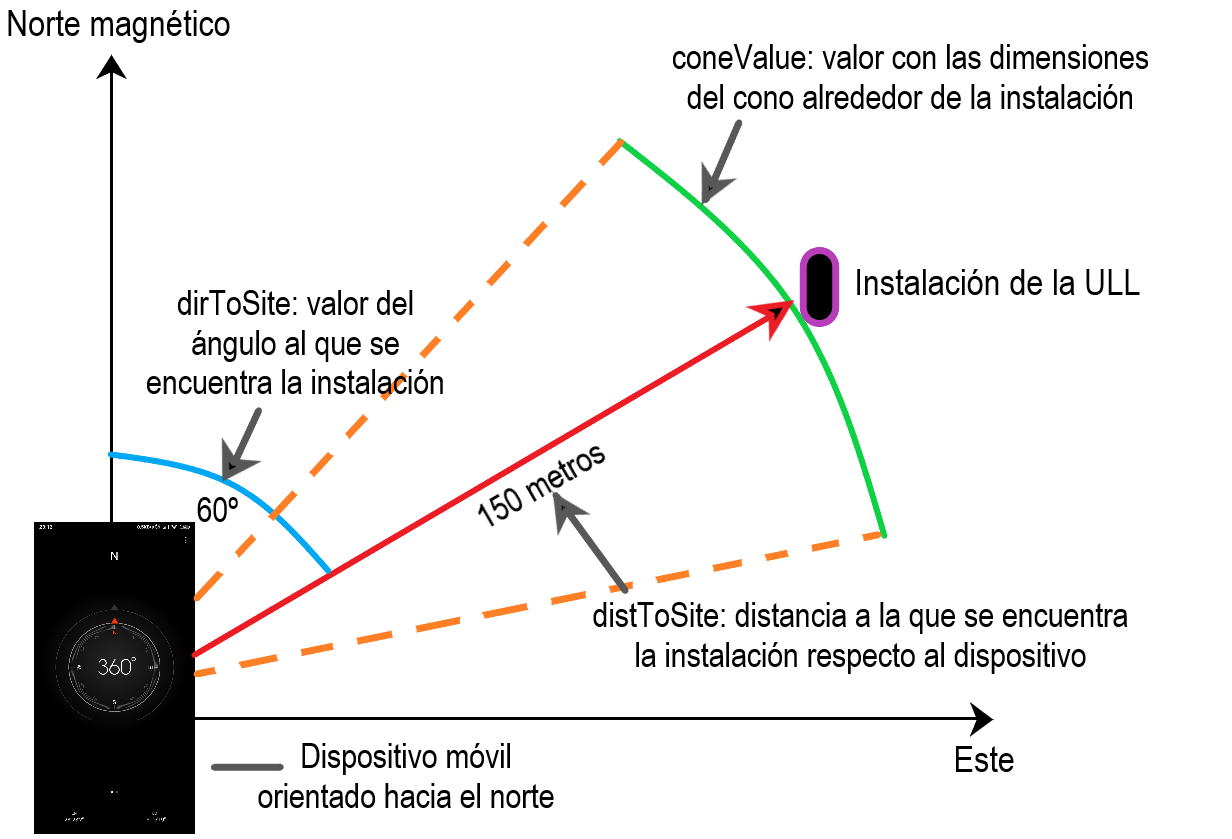
\includegraphics[width=0.65\linewidth]{Images/imagenAR}
			\end{center}
\end{frame}
 
\begin{frame}
	\frametitle{Modelos encargados de la navegación}
			\block{\texttt{Navigation.java}}
			\begin{itemize}
				\item Clase encargada de identificar las instalaciones.
				\item Contiene una lista con todas las instalaciones.
				\item Recibe los datos de los sensores.
				\item Calcula la distancia, dirección y valor de cono para cada instalación.
			\end{itemize}
			\endblock{}
\end{frame}
 
 
\begin{frame}
	\frametitle{Atributos de la clase \texttt{Navigation.java}}
	\lstinputlisting{Code/navigation1.java}
\end{frame}

\begin{frame}
	\frametitle{Métodos de la clase\texttt{Navigation.java}}
	\lstinputlisting{Code/navigation2.java}
\end{frame}

\begin{frame}
	\frametitle{Método calculateCone(double dist)}
	\lstinputlisting{Code/navigation3.java}
\end{frame}
	  
\begin{frame}
	\frametitle{\texttt{Navigation.java}}
	\lstinputlisting{Code/navigation4.java}
	\lstinputlisting{Code/navigation5.java}
\end{frame}

     
\begin{frame}
	\frametitle{whatCanSee(LatLng currentPosAux, double actualDir)}
	\lstinputlisting{Code/navigation6.java}
\end{frame}
\begin{frame}
	\frametitle{whatCanSee(LatLng currentPosAux, double actualDir)}
	\lstinputlisting{Code/navigation7.java}
\end{frame}


\begin{frame}
	\frametitle{Modo de Realidad Aumentada}
			\block{Obtención de la información}
			\begin{itemize}
				\item La información de las instalaciones la provee el servidor que a su vez se comunica con la base de datos.
				\item La clase \texttt{GetData.java} se encarga de conectar con el servidor y manejar la respuesta.
				\item Los radios máximos y minimos con los que identificar las instalaciones están guardados en las Shared Preferences.
			\end{itemize}
			\endblock{}
\end{frame}

\begin{frame}
	\frametitle{\texttt{GetData.java}}
	\lstinputlisting{Code/getdata.java}
\end{frame}

\begin{frame}
	\frametitle{Métodos encargados de la obtención de la información}
	\lstinputlisting{Code/getdata2.java}
	\lstinputlisting{Code/getdata3.java}
\end{frame}

\begin{frame}
	\frametitle{Modo de Realidad Aumentada}
	\begin{columns}
		\begin{column}{0.6\textwidth}
			\block{Visualización}
			\begin{itemize}
				\item El activity ``ARNavigation'' es el encargado de la visualización de la técnica de RA.
				\item Este activity hereda de la clase ``ARActivity'' del SDK de Kudan.
			\end{itemize}
			\endblock{}
		\end{column}
		\begin{column}{0.4\textwidth} 
			\vfill 
			\begin{center}
				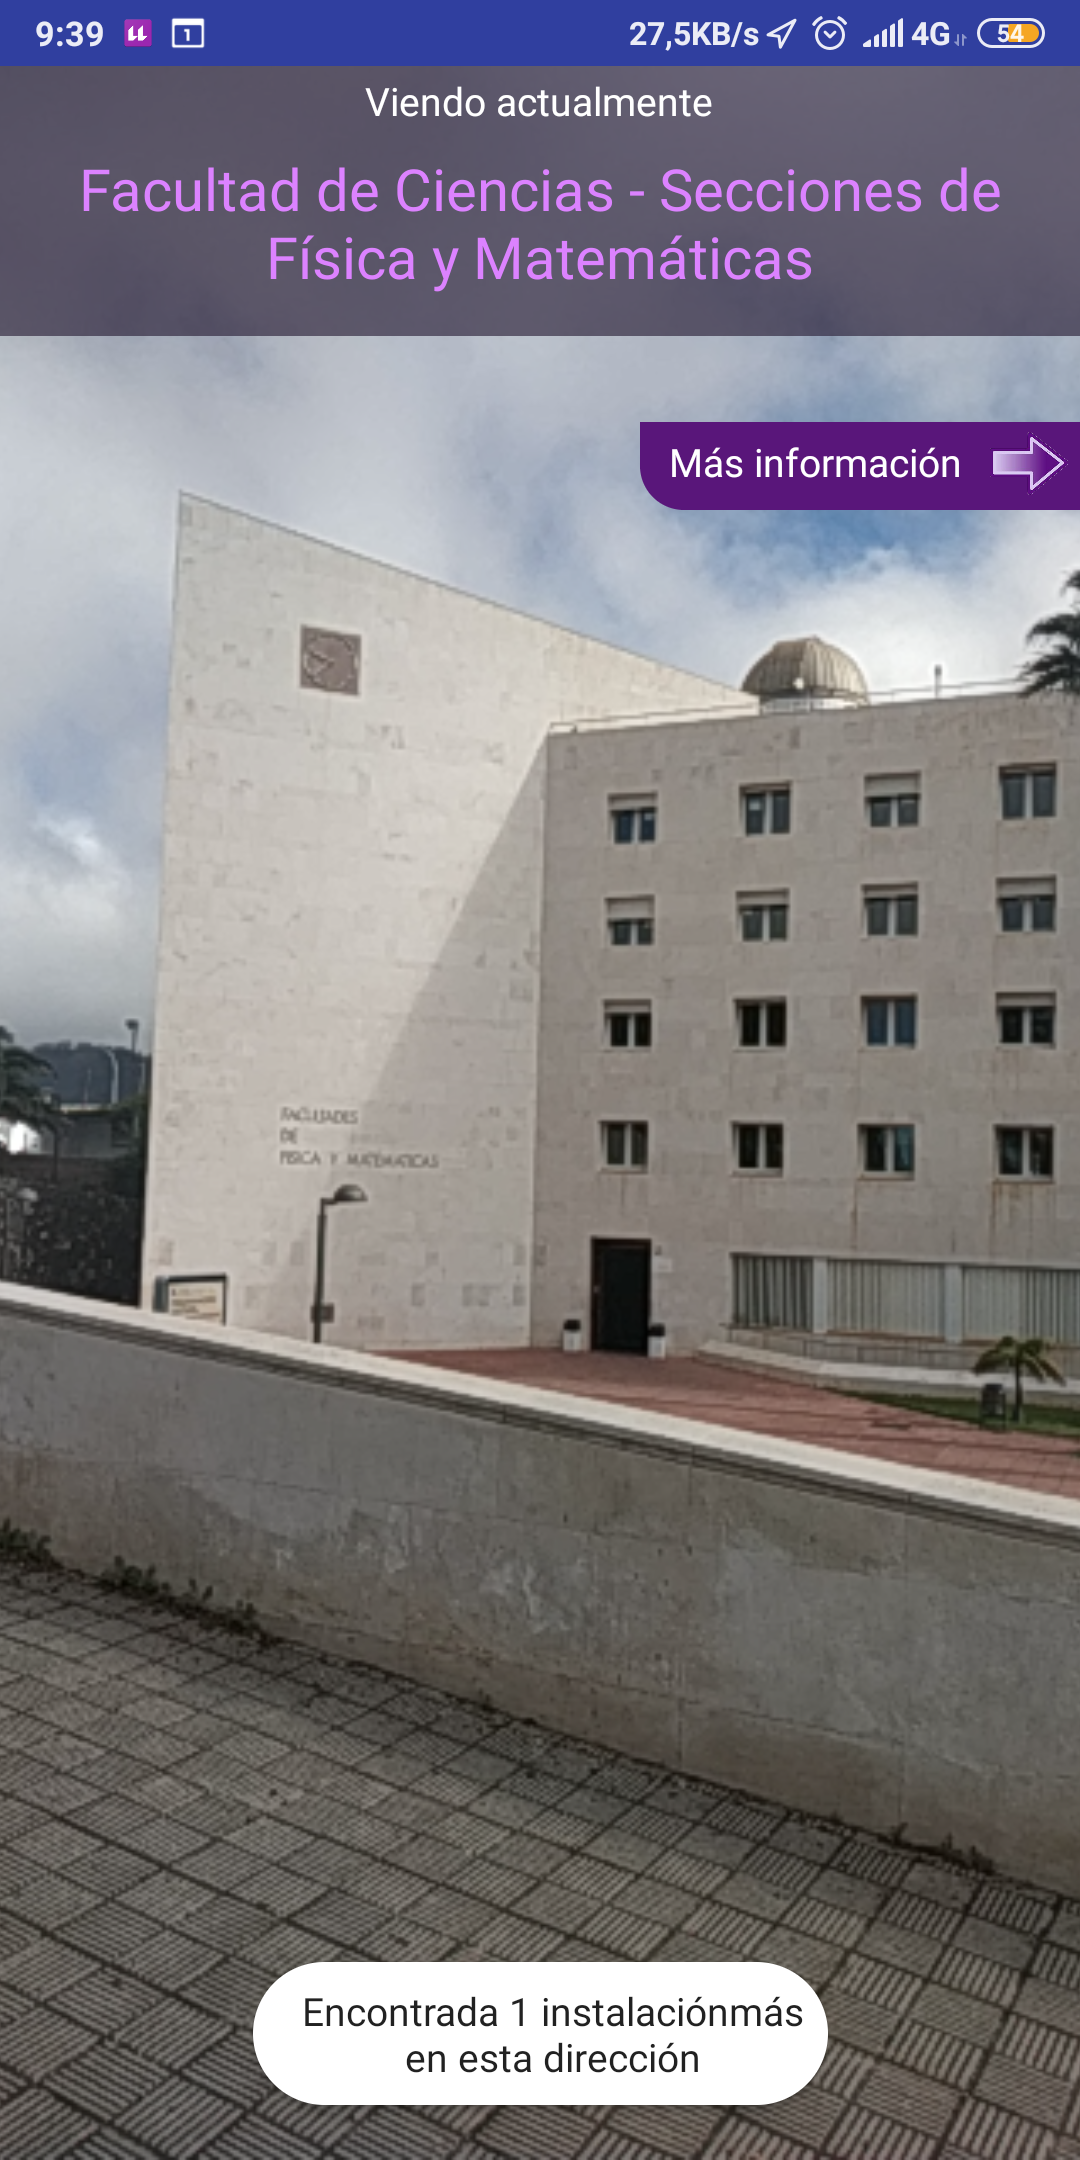
\includegraphics[width=0.7\linewidth]{Images/ar}
			\end{center}
		\end{column}
	\end{columns}
\end{frame}

\begin{frame}
	\frametitle{\texttt{arnavigation.xml}}
	\lstinputlisting{Code/visualizacion.xml}
\end{frame}

\begin{frame}
	\frametitle{Fragmentos de \ULLAR{}}
			\block{Fragmentos en Android}
			\begin{itemize}
				\item ¿Qué es un fragmento?
				\item ¿Qué beneficios ofrecen para la aplicación?
				\item Fragmentos de \ULLAR{}:
				\begin{itemize}
					\item MapsFragment.
					\item HomeFragment.
					\item AboutFragment.
				\end{itemize}
			\end{itemize}
			\endblock{}

\end{frame}

    

\begin{frame}
	\frametitle{Fragmentos de \ULLAR{}}
	\begin{columns}
		\begin{column}{0.6\textwidth}
			\block{MapsFragment}
			\begin{itemize}
				\item Nos proporciona un mapa generado por la API de Google Maps.
				\item En este mapa permite:
				\begin{itemize}
					\item Dibujar las instalaciones de la ULL.
					\item Ubicar al dispositivo.
					\item Dibujar dos circunferencias que actuan como rango de aparición de las instalaciones. 
				\end{itemize}
			\end{itemize}
			\endblock{}
		\end{column}
		\begin{column}{0.4\textwidth} 
			\vfill 
			\begin{center}
				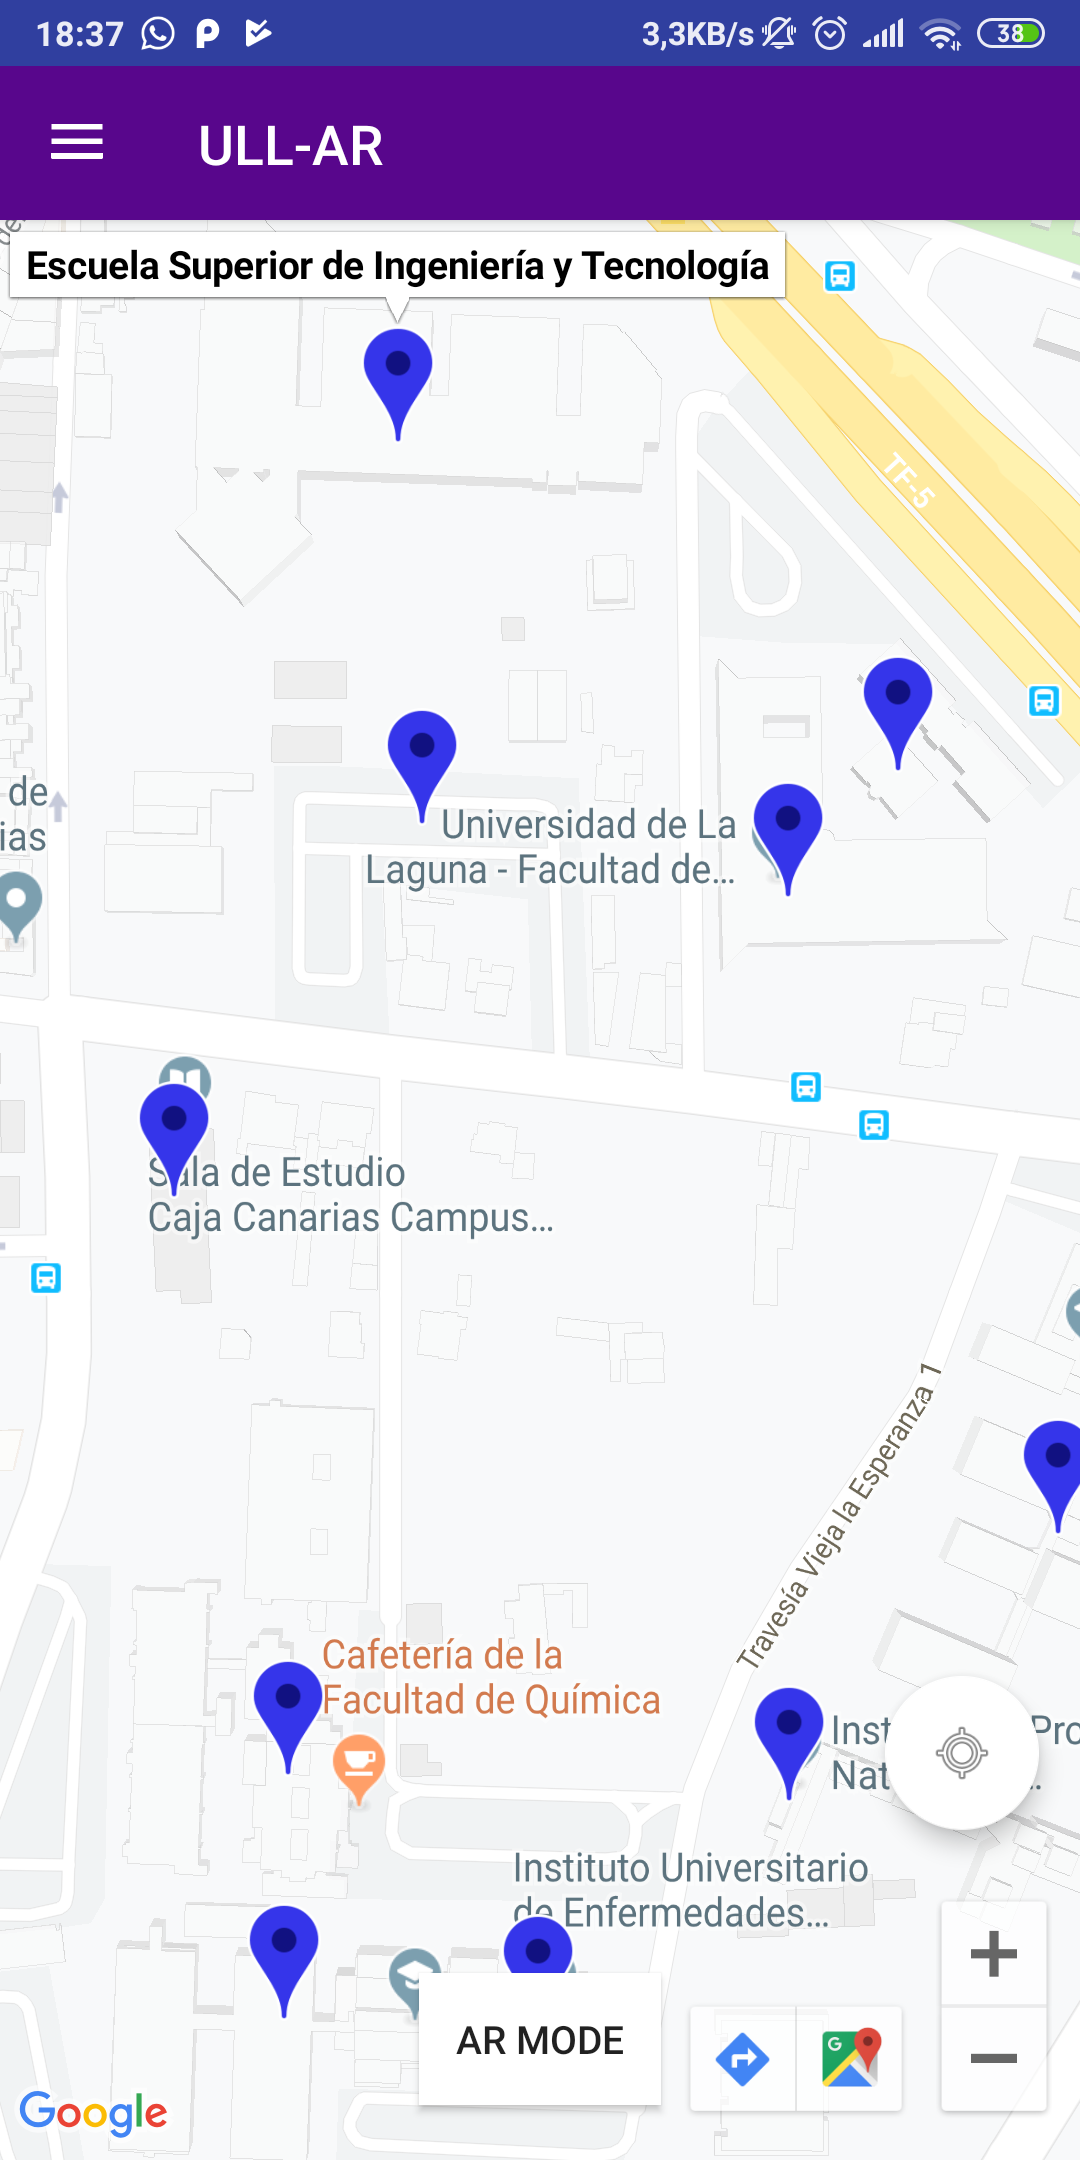
\includegraphics[width=0.7\linewidth]{Images/mapsApp}
			\end{center}
		\end{column}
	\end{columns}
\end{frame}


\begin{frame}
	\frametitle{\texttt{MapsFragment.java}}
	\lstinputlisting{Code/mapsfragment.java}
\end{frame}



\begin{frame}
	\frametitle{\texttt{fragment\_maps.xml}}
	\lstinputlisting{Code/fragmentmaps.xml}
\end{frame}

\begin{frame}
	\frametitle{Fragmentos de \ULLAR{}}
	\begin{columns}
		\begin{column}{0.6\textwidth}
			\block{HomeFragment}
			\begin{itemize}
				\item Primera vista que aparece cuando el usuario se autentifica en la aplicación.
				\item Uso del modelo de ``RecyclerView'' y adaptadores de Android.
				\item La clase ``ItemHome'' contiene los atributos a mostrar.
			\end{itemize}
			\endblock{}
		\end{column}
		\begin{column}{0.4\textwidth} 
			\vfill 
			\begin{center}
				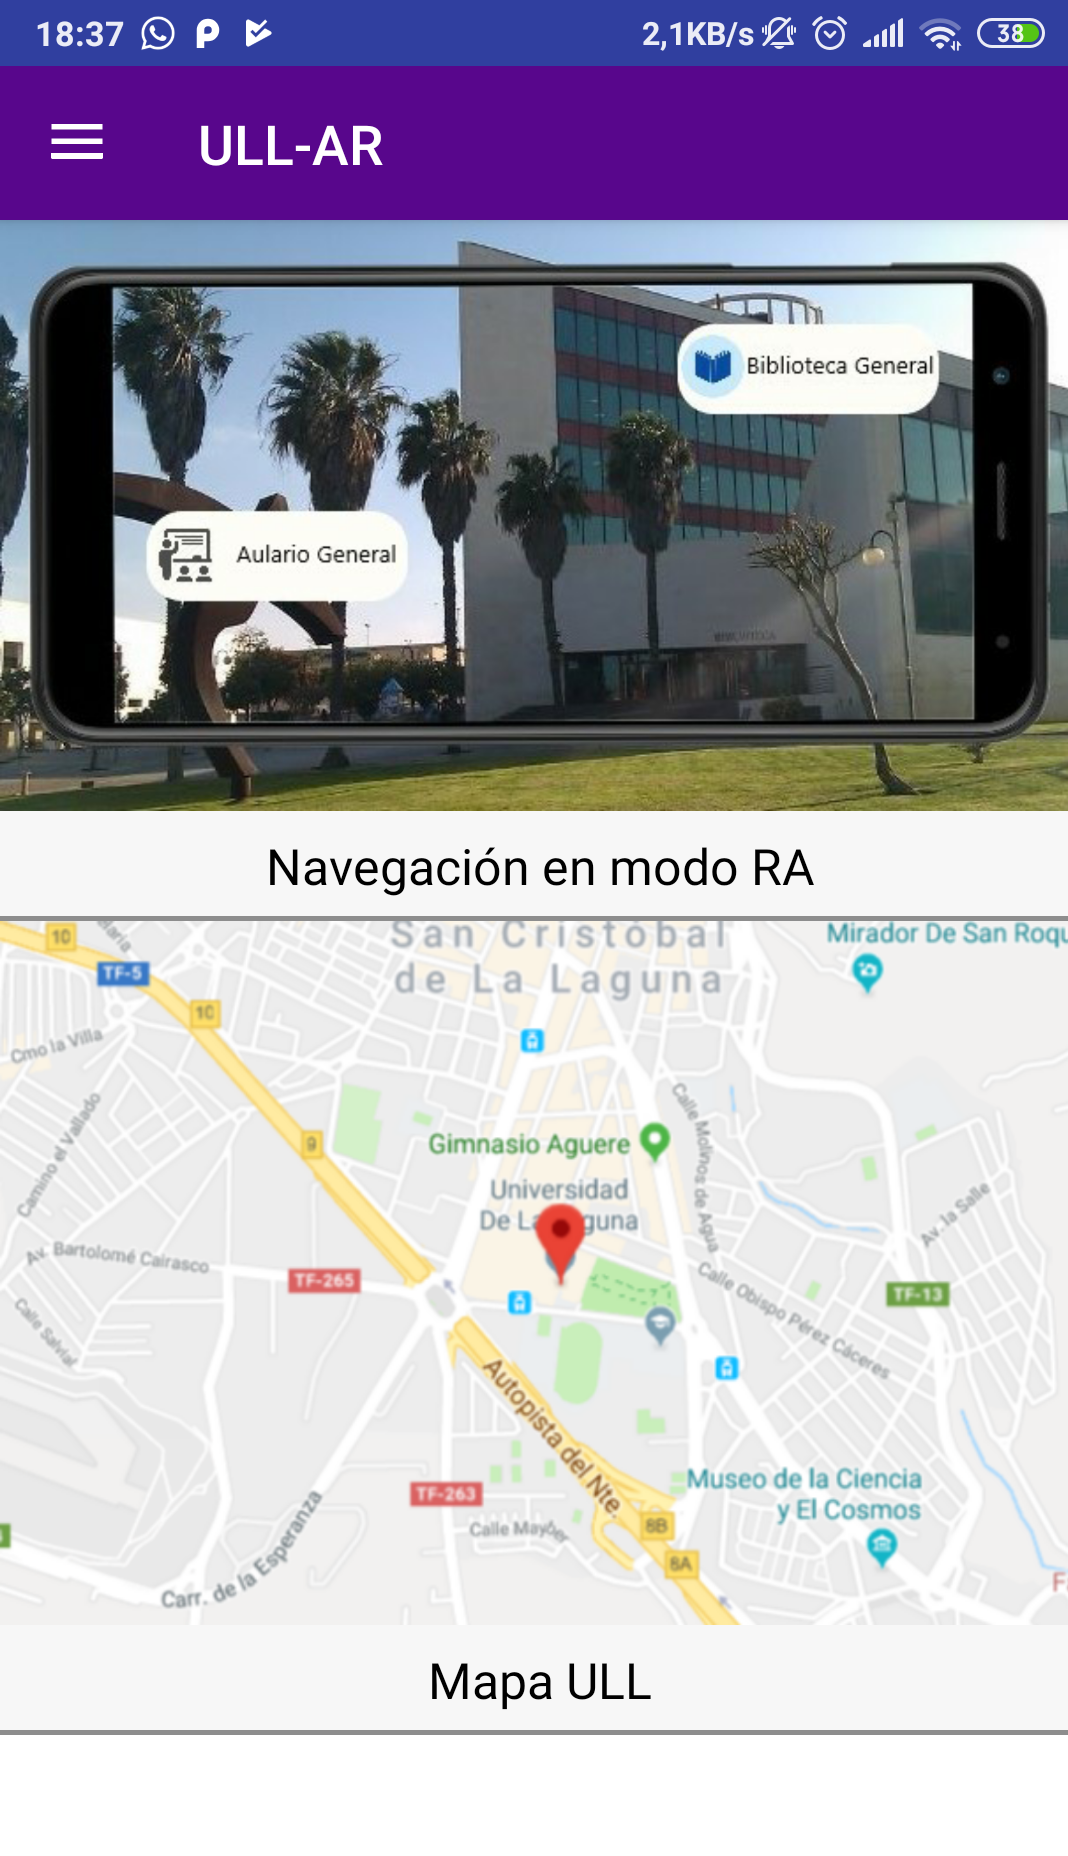
\includegraphics[width=0.8\linewidth]{Images/homeApp}
			\end{center}
		\end{column}
	\end{columns}
\end{frame}

         
      
\begin{frame}
	\frametitle{\texttt{ItemHomeAdapter.java}}
	\lstinputlisting{Code/homefragment1.java}
\end{frame}

         

\begin{frame}
	\frametitle{\texttt{HomeFragment.java}}
	\lstinputlisting{Code/homefragment2.java}
\end{frame}

\begin{frame}
	\frametitle{\texttt{fragment\_home.xml}}
	\lstinputlisting{Code/homefragment3.xml}
\end{frame}


\begin{frame}
	\frametitle{Fragmentos de \ULLAR{}}
	\begin{columns}
		\begin{column}{0.6\textwidth}
			\block{AboutFragment}
			\begin{itemize}
				\item Información general de la aplicación:
				\begin{itemize}
					\item Nombre.
					\item Autor.
					\item Version.
					\item Email.
					\item Descripción de la aplicación.
				\end{itemize}
			\end{itemize}
			\endblock{}
		\end{column}
		\begin{column}{0.4\textwidth} 
			\vfill 
			\begin{center}
				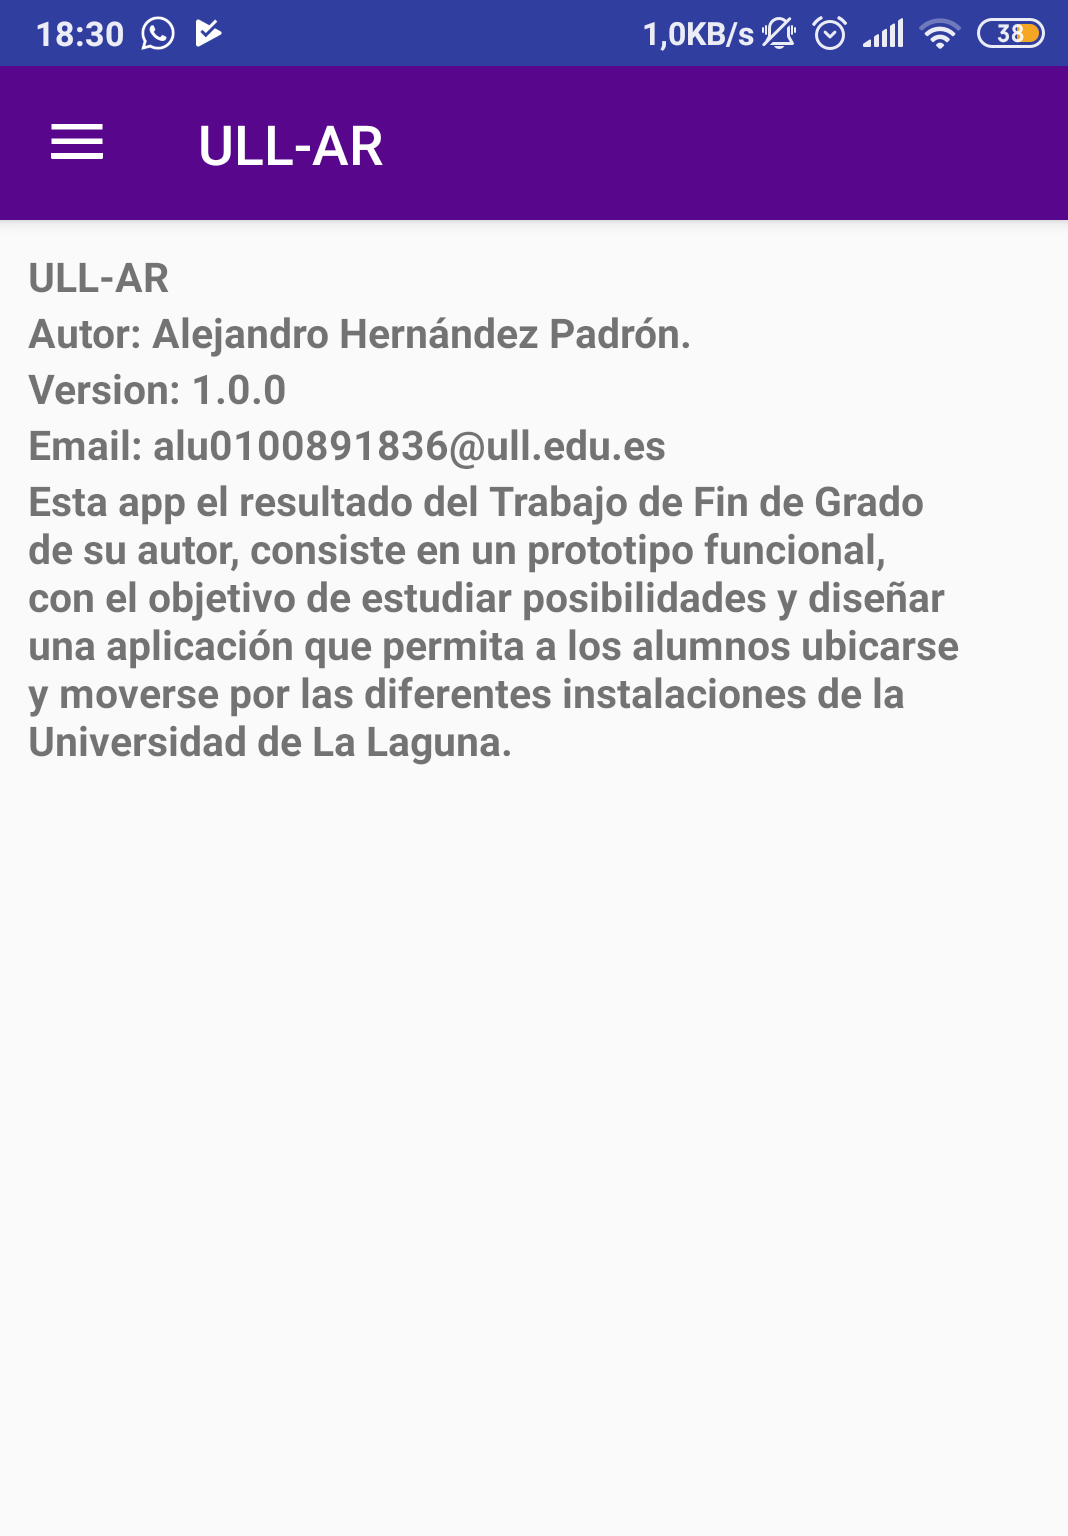
\includegraphics[width=0.8\linewidth]{Images/infoApp}
			\end{center}
		\end{column}
	\end{columns}
\end{frame}


\begin{frame}
	\frametitle{Menú de \ULLAR{}}
	\begin{columns}
		\begin{column}{0.6\textwidth}
			\block{Navigation Drawer}
			\begin{itemize}
				\item ¿Qué es un menú Navigation Drawer?.
				\item Se encuentra en multitud de aplicaciones.
				\item Mejor apariencia.
				\item Velocidad de carga entre fragmentos.
				\item La clase ``BaseActivity.java'' incorpora esté menú.
			\end{itemize}
			\endblock{}
		\end{column}
		\begin{column}{0.4\textwidth} 
			\vfill 
			\begin{center}
				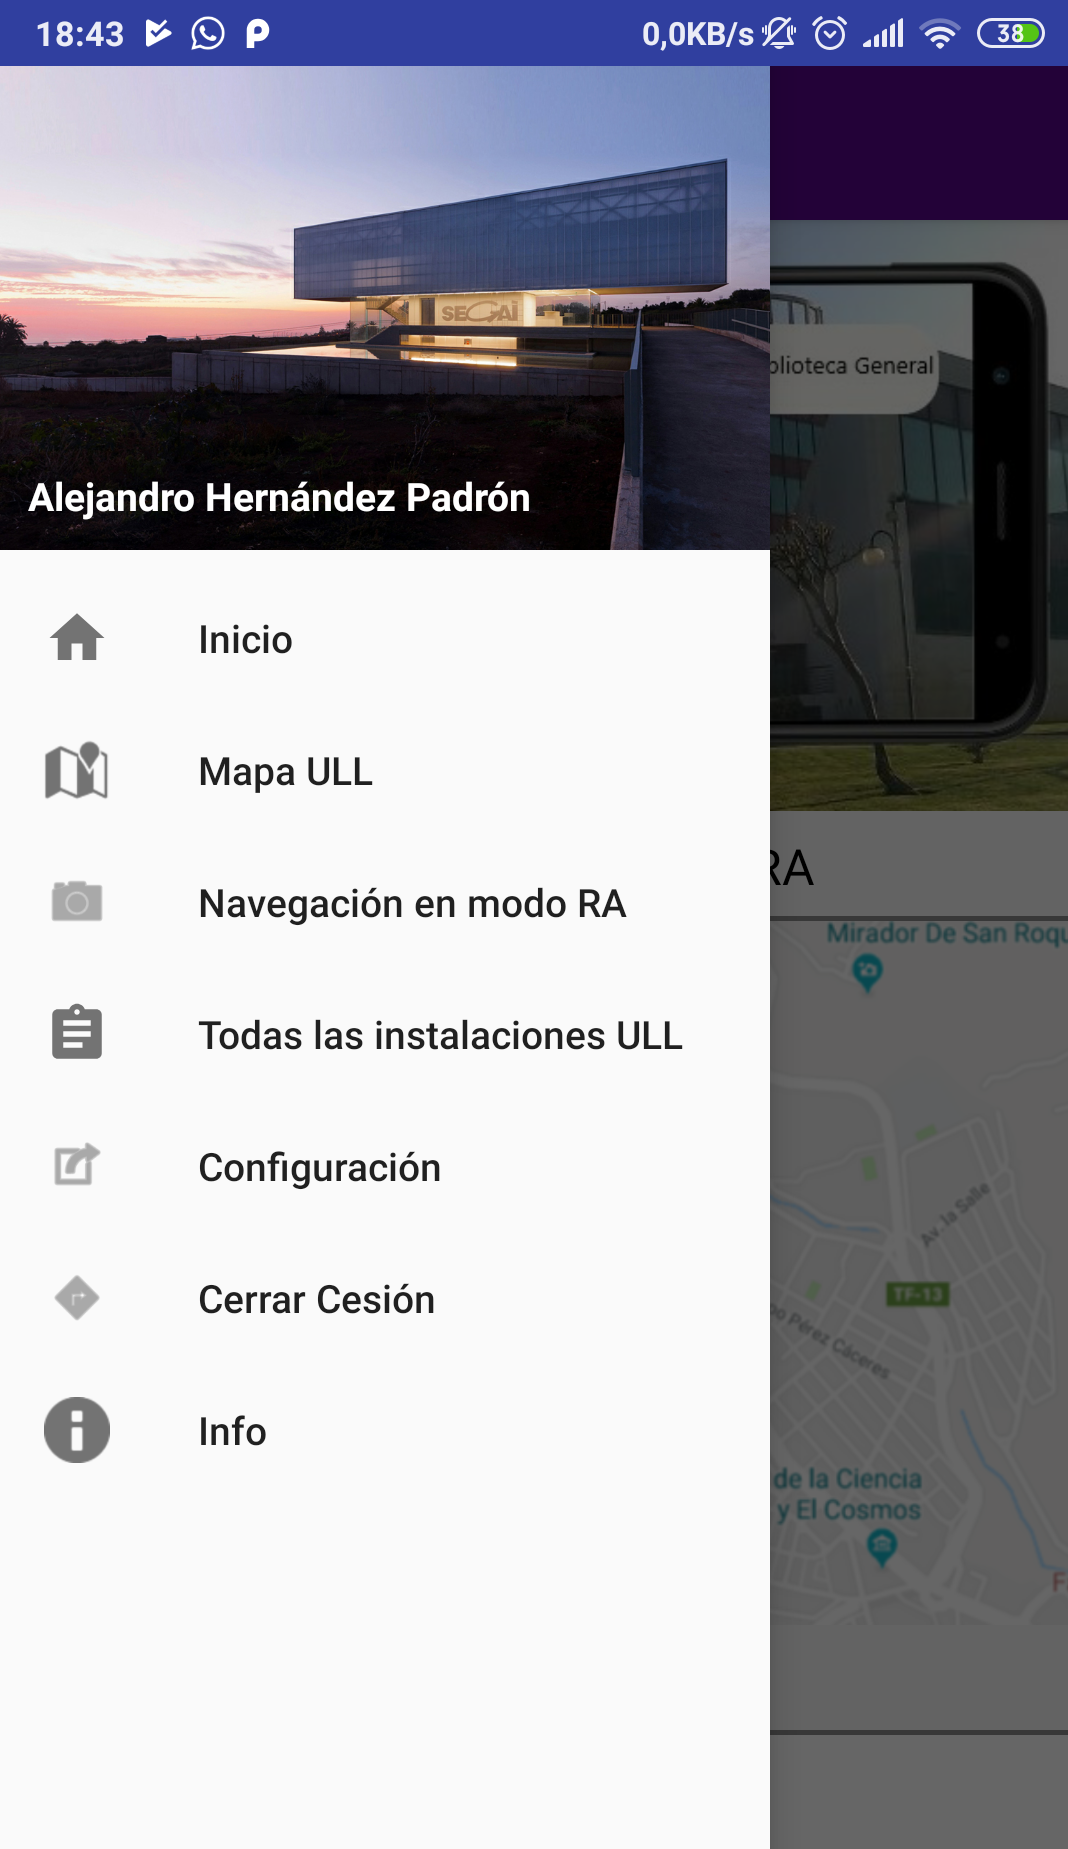
\includegraphics[width=0.8\linewidth]{Images/menuApp}
			\end{center}
		\end{column}
	\end{columns}
\end{frame}



\begin{frame}
	\frametitle{\texttt{navigation\_draw.xml}}
	\lstinputlisting{Code/menu1.xml}
\end{frame}


\begin{frame}
	\frametitle{\texttt{nav\_options.xml}}
	\lstinputlisting{Code/menu2.xml}
\end{frame} 
 

\begin{frame}
	\frametitle{\texttt{BaseActivity.java}}
	\lstinputlisting{Code/menu3.java}
\end{frame} 
 
 

\begin{frame}
	\frametitle{Instalaciones de la ULL}
	\begin{columns}
		\begin{column}{0.6\textwidth}
			\block{Ventana de \textit{Todas las instalaciones}}
			\begin{itemize}
				\item Permite al usuario acceder a las instalaciones de la BD.
				\item Realizar una busqueda.
				\item Uso de adaptadores para mostrar información básica de cada instalación.
				\item Permite acceder a la ficha de información de cada instalación.
			\end{itemize}
			\endblock{}
		\end{column}
		\begin{column}{0.4\textwidth} 
			\vfill 
			\begin{center}
				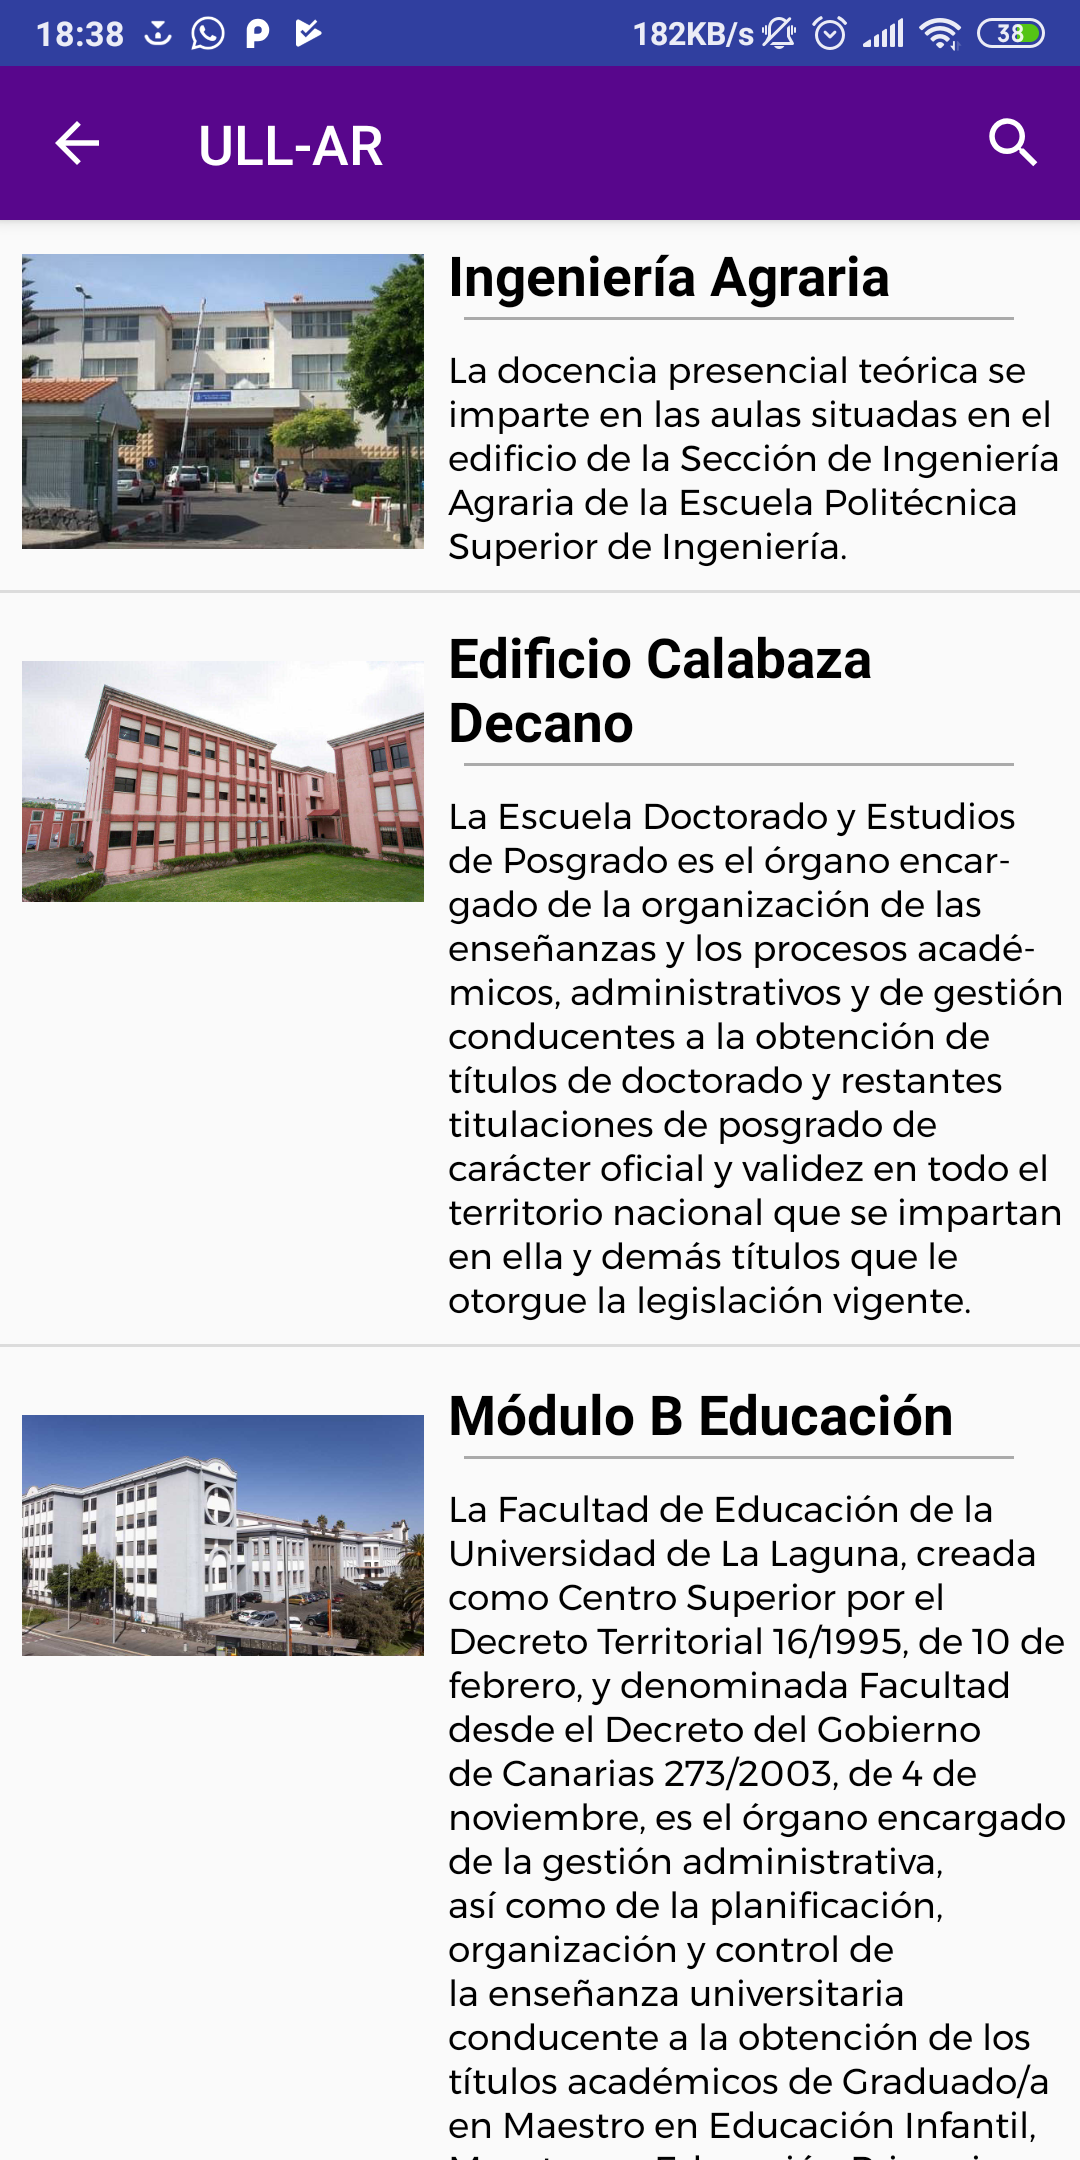
\includegraphics[width=0.75\linewidth]{Images/allSitesApp}
			\end{center}
		\end{column}
	\end{columns}
\end{frame} 
  

\begin{frame}
	\frametitle{\texttt{SiteAdapter.java}}
	\lstinputlisting{Code/instalaciones1.java}
\end{frame} 
 

\begin{frame}
	\frametitle{\texttt{SitesListActivity.java}}
	\lstinputlisting{Code/instalaciones2.java}
\end{frame}  

\begin{frame}
	\frametitle{\texttt{SitesListActivity.java}}
	\lstinputlisting{Code/instalaciones3.java}
\end{frame}  


\begin{frame}
	\frametitle{Instalaciones de la ULL}
	\begin{columns}
		\begin{column}{0.6\textwidth}
			\block{Ventana de \textit{Información de la instalación}}
			\begin{itemize}
				\item Muestra información detallada de la instalación.
				\item Permite acceder a la ruta a de la instalación en Google Maps.
				\item Muestra los enlaces de interes relacionados.
			\end{itemize}
			\endblock{}
		\end{column}
		\begin{column}{0.4\textwidth} 
			\vfill 
			\begin{center}
				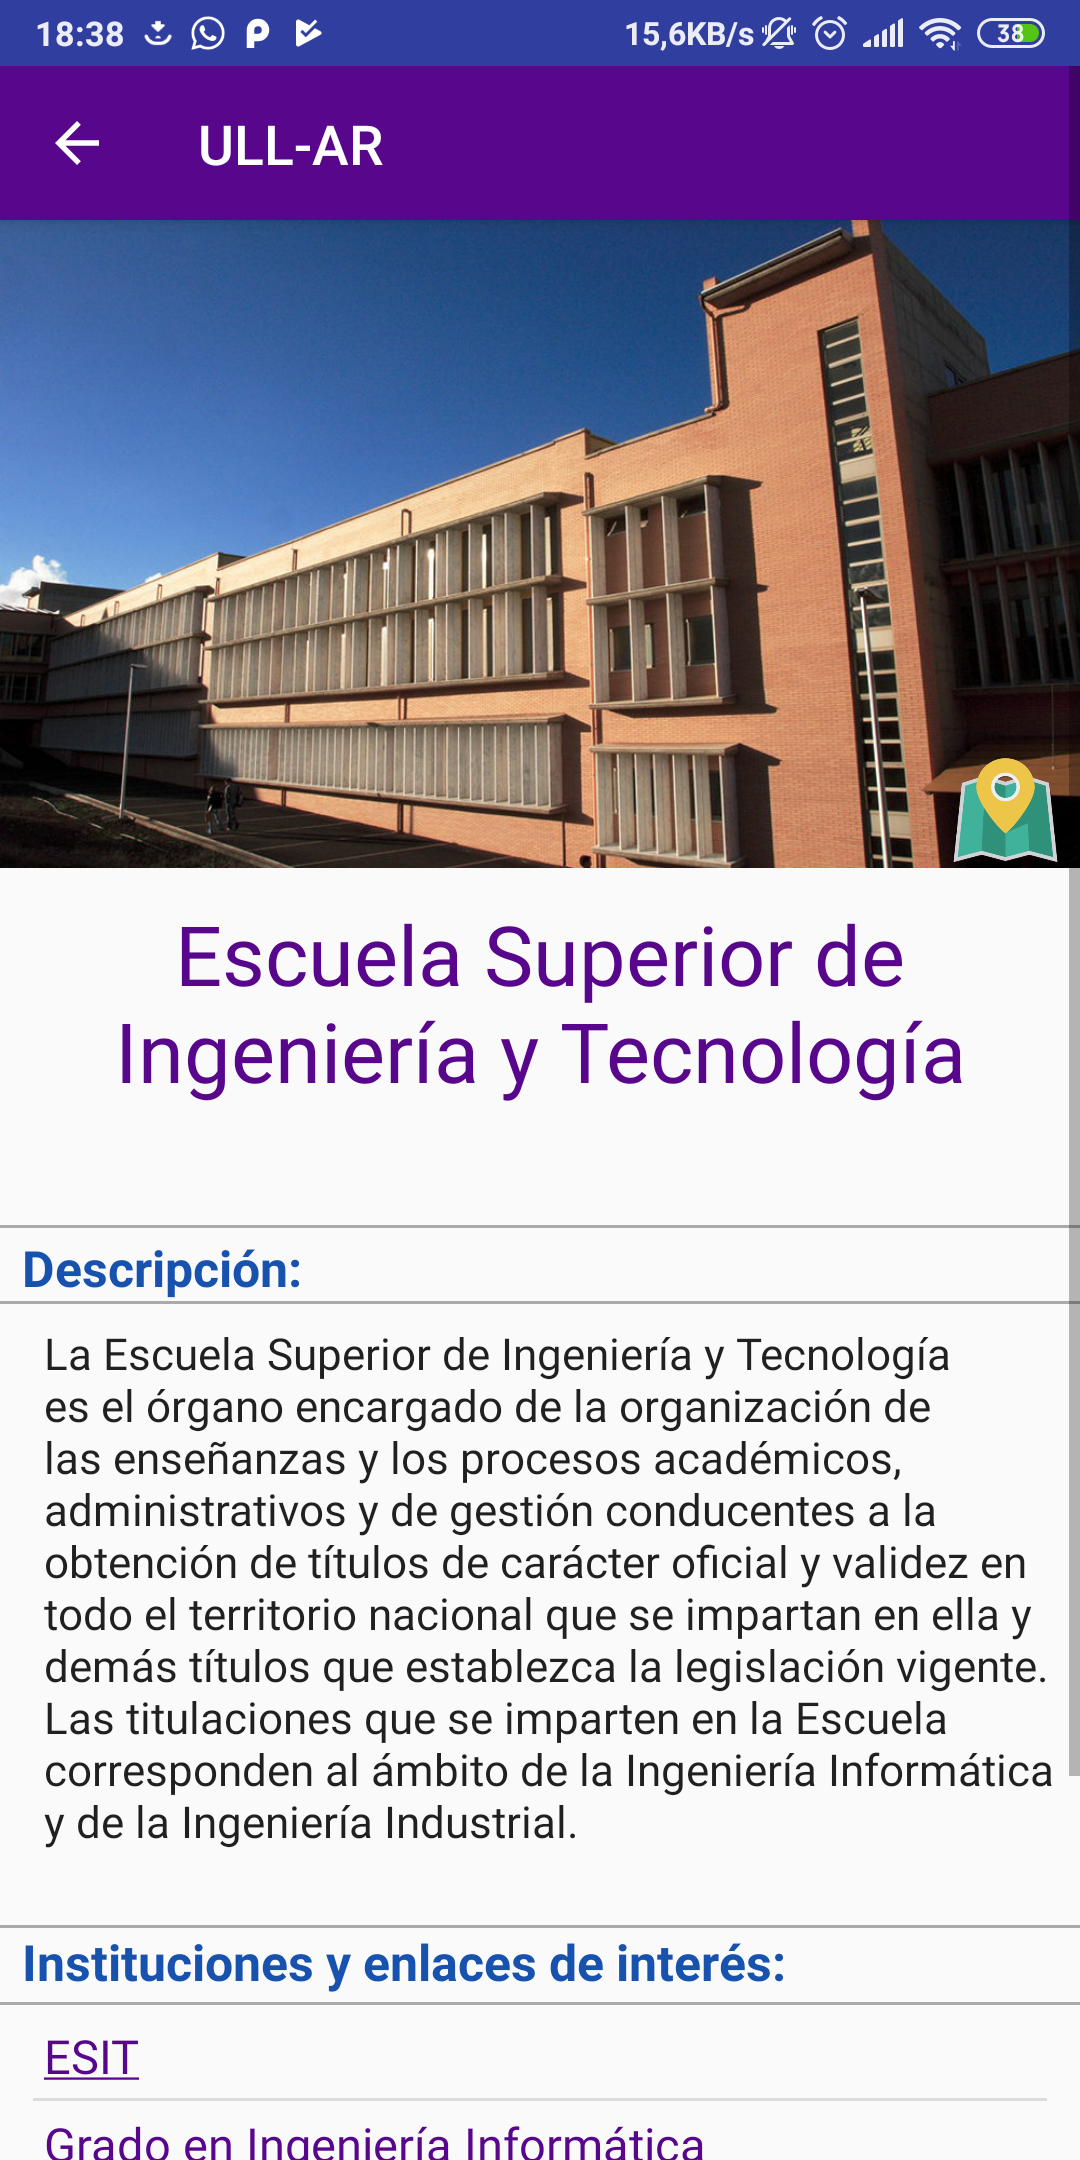
\includegraphics[width=0.75\linewidth]{Images/siteInfoApp}
			\end{center}
		\end{column}
	\end{columns}
\end{frame} 
  
\begin{frame}
	\frametitle{\texttt{SiteDescriptionActivity.java}}
	\lstinputlisting{Code/instalaciones4.java}
\end{frame}  


\begin{frame}
	\frametitle{Preferencias del usuario}
	\begin{columns}
		\begin{column}{0.6\textwidth}
			\block{Ventana de \textit{Información de la instalación}}
			\begin{itemize}
				\item Ventana donde van los ajustes de la aplicación
				\item Se pueden configurar los radios de busqueda de las instalaciones.
			\end{itemize}
			\endblock{}
		\end{column}
		\begin{column}{0.4\textwidth} 
			\vfill 
			\begin{center}
				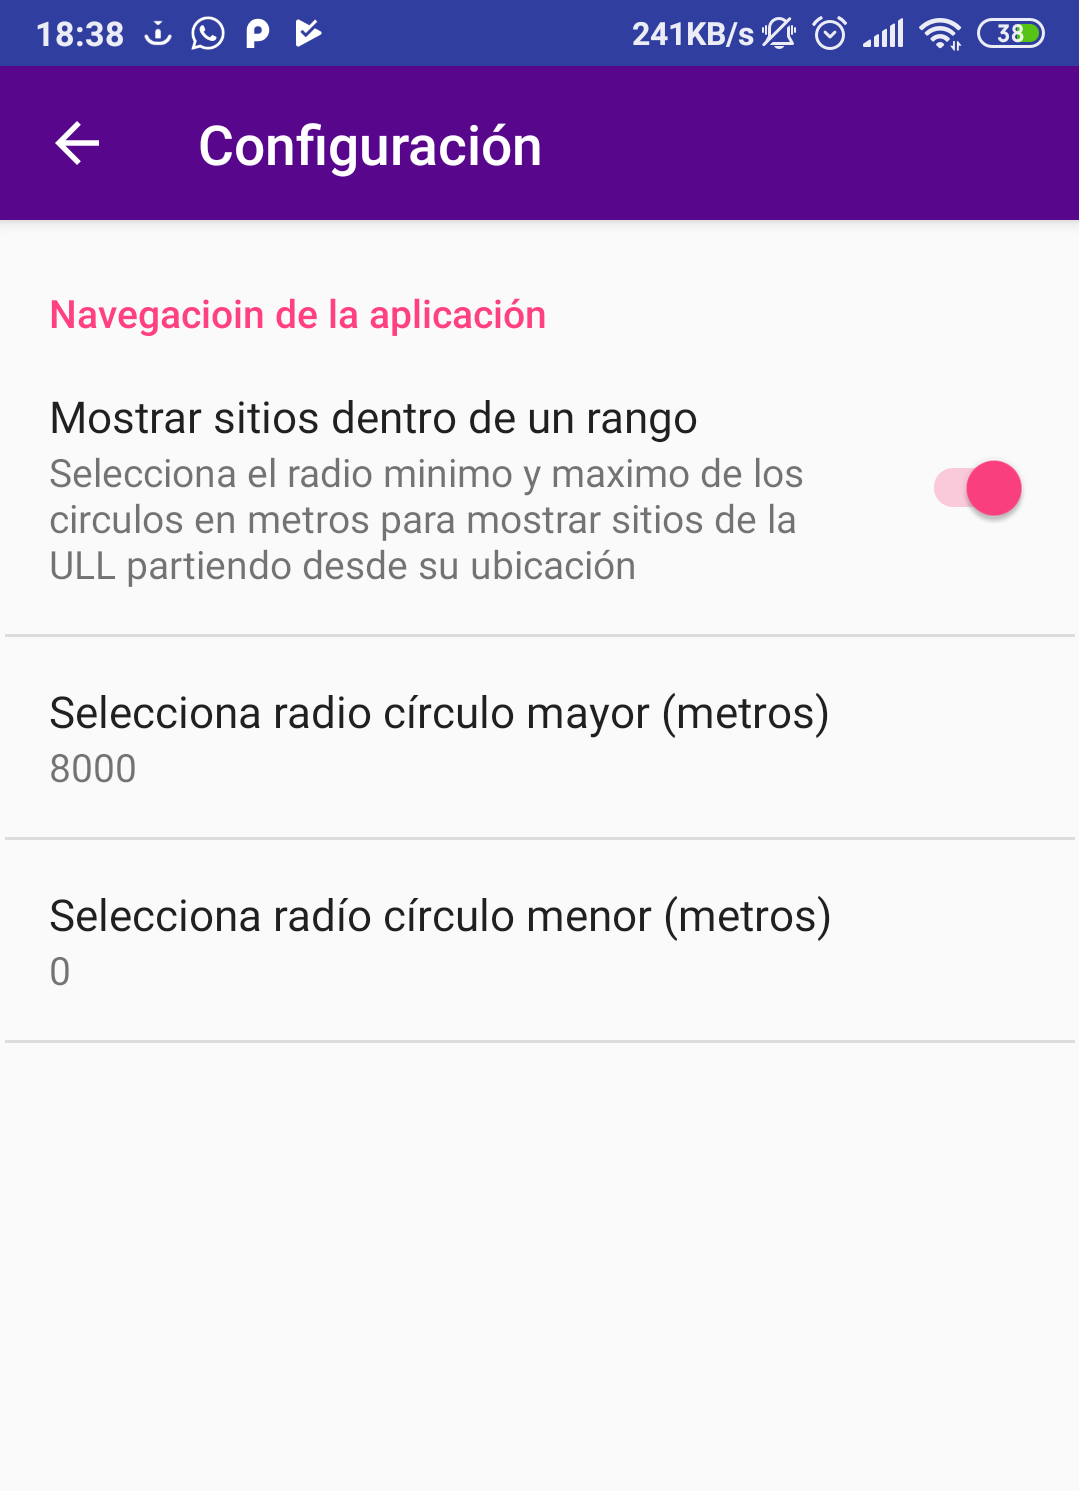
\includegraphics[width=0.9\linewidth]{Images/settingsApp}
			\end{center}
		\end{column}
	\end{columns}
\end{frame} 

\begin{frame}
	\frametitle{\texttt{SiteAdapter.xml}}
	\lstinputlisting{Code/settings.xml}
\end{frame}  
%----------------- ---------------------------------------------------
